\documentclass[conference]{IEEEtran}
\IEEEoverridecommandlockouts
% The preceding line is only needed to identify funding in the first footnote. If that is unneeded, please comment it out.
\usepackage{cite}
\usepackage{amsmath,amssymb,amsfonts}
\usepackage{algorithmic}
\usepackage{graphicx}
\usepackage{textcomp}
\usepackage{xcolor}
\def\BibTeX{{\rm B\kern-.05em{\sc i\kern-.025em b}\kern-.08em
    T\kern-.1667em\lower.7ex\hbox{E}\kern-.125emX}}
\begin{document}

\title{Alternative Optimization Methods for Neural Networks}

\author{\IEEEauthorblockN{Abdullah Bilici}
\IEEEauthorblockA{\textit{Istanbul Technical University} \\
150200330 \\
bilicia20@itu.edu.tr}
\and
\IEEEauthorblockN{Eren Oluğ}
\IEEEauthorblockA{\textit{Istanbul Technical University} \\
150200333 \\
olug20@itu.edu.tr}
\and
\IEEEauthorblockN{Salim Beyden}
\IEEEauthorblockA{\textit{Istanbul Technical University} \\ 150200307 \\
beyden20@itu.edu.tr}
}

\maketitle

\begin{abstract}
In this project, our aim is to evaluate the efficiency of various gradient-free optimization methods, we worked with Genetic Algorithms (GA) and Simulated Annealing (SA), for improving the training of neural networks. Our focus was on investigating how these methods can be employed individually or in combination with gradient methods such as Gradient Descent to optimize the training process. The project is include researching and implementing these optimization techniques, assessing the performance and effectiveness of neural network training tasks in compared to more conventional gradient-based approaches.
\end{abstract}

\begin{IEEEkeywords}
optimization, neural, network, simulated, annealing, genetic
\end{IEEEkeywords}

\section{\textbf{Describing The Problem}}

In general, gradient-based methods are widely used for traning neural network because of the their effective process. On the other hand, they have some problems in certain situations like stucking in local optima, dealing with non-differentiable or discontinuous functions,high-dimensional search spaces, automate hyperparameter tuning. In these situations, gradient-free methods can be more useful. So, we will looking for possible solutions for these problems in this project.

\section{\textbf{Methods}}

\subsection{Gradient Descent}
Gradient Descent is an optimization algorithm commonly used to minimize the cost or loss function of a machine learning model. It is particularly applied in training neural networks. The basic idea behind Gradient Descent is to iteratively update the model's parameters in the direction of the steepest descent of the cost function, with the aim of reaching the global or local minimum.

\begin{figure}[h]
    \centering
    \label{Gradient Descent}
\end{figure}

\begin{center}
    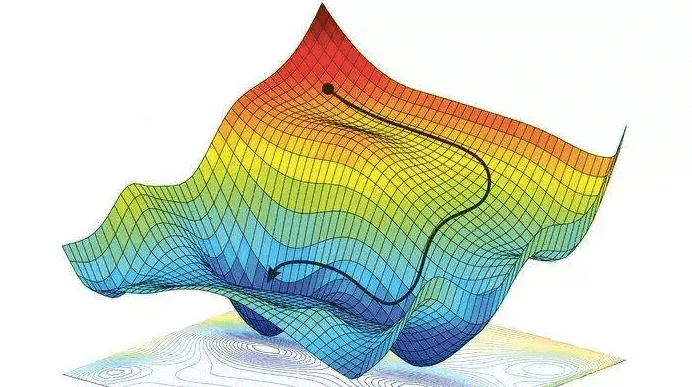
\includegraphics[width=6.5cm]{gradient_descent.png}\\ 
    \footnotesize{Gradient Descent [1]}
\end{center}\\ 

\noindent \textbf{Steps of the Gradient Descent:}
\begin{itemize}
    \item \textbf{Objective:} \\
    In neural network optimization, the goal is to reduce the cost or loss function, which evaluates the difference between the network's predicted outputs and the actual outputs of the training set.
    
    \item \textbf{Parameter Update:} \\
    Gradient Descent updates the neural network's parameters (weights and biases) iteratively in the direction of the cost function's steepest descent. The goal is to identify the parameters ideal values, which minimize the cost function.
    
    \item \textbf{Gradient Calculation:} \\
     The key step in Gradient Descent is to calculate the gradient of the cost function with respect to each parameter. The gradient represents the direction and magnitude of the steepest ascent in the cost function space. By negating the gradient, the algorithm moves in the direction of the steepest descent, effectively reducing the cost function.
    
    \item \textbf{Learning Rate:} \\
    The learning rate is a hyperparameter that determines the step size taken in each iteration of Gradient Descent. It controls how much the parameters are adjusted based on the gradient. A larger learning rate may lead to faster convergence, but it can also cause overshooting the optimal solution. A smaller learning rate may result in slower convergence but with more precise parameter updates.
    
    \item \textbf{Parameter Update Equation:} \\
    The following equation is used to update the parameters in Gradient Descent:
    $$
    \theta_{\text{new}} = \theta_{\text{old}} - \alpha \nabla J(\theta_{\text{old}})
    $$
    where;
    $$
    \theta_{\text{new}}: \text{New Parameter}
    $$
    $$
    \theta_{\text{old}}: \text{Old Parameter}
    $$
    $$
    \alpha: \text{Learning Rate}
    $$
    $$
    \nabla J(\theta_{\text{old}}): \text{Gradient of the Cost Function, respect to } \theta_{\text{old}}
    $$
    
    \item \textbf{Batch and Stochastic Gradient Descent:} \\
    There are variations of Gradient Descent based on the size of the data used for gradient calculation. In batch gradient descent, the gradient is calculated using the entire training dataset, which can be computationally expensive. In stochastic gradient descent, the gradient is computed using a single randomly selected sample from the dataset, which can be more computationally efficient but may introduce more noise in the parameter updates. Mini-batch gradient descent is a compromise between these two approaches, where the gradient is computed using a small subset (mini-batch) of the training data.
\end{itemize}

\subsection{Simulated Annealing}
Simulated Annealing is a meta-heuristic algorithm that draws inspiration from the metallurgical annealing procedure. It is commonly used to solve combinatorial optimization problems where the goal is to find the best solution among a vast number of possible solutions.

Simulated annealing contains a probabilistic element by accepting worse solutions than the current one to escape the local optima. This decision mecanism is controlled by a temperature parameter which decreases through iterations. Initially, since the temperature parameter is high, the method is more likely to accept worse solutions, but as the temperature decreases, it becomes more likely to be only accepting better solutions.
\begin{center}
    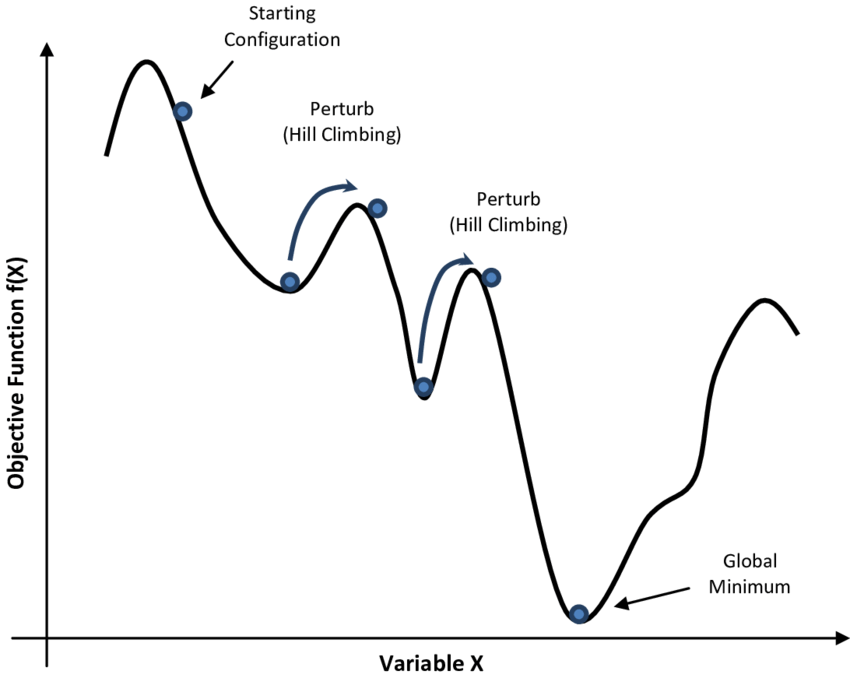
\includegraphics[width=7cm]{sa_1.png}\\ \ \\
    \footnotesize{Simulated Annealing [2]}
\end{center}\\ 


The classic acceptance criterion of SA comes from statistical mechanics, and it is based on the Boltzmann probability distribution. A system in thermal equilibrium at temperature T can be found in a state with energy E with a probability proportional to $\exp (-E / k T)$.
\begin{center}
    $Prob(E) \sim \exp(-E/kT)$
\end{center}
where the $k$ is the Boltzmann constant.

TSP problem, clustering, feature selection, neural network training, hyperparameter tuning and optimization of model parameters are some example use of simulated annealing algorithm. The flexibility and robustness of method.


\pagebreak
\subsection{Genetic Algorithm}

The genetic algorithm is a powerful optimization technique. It is widely used to solve complex problems where traditional algorithms may be inefficient or impractical..

The genetic algorithm mimics the principles of natural selection. It works by maintaining a population of potential solutions, evolving them over generations to find the best solution. The key components of a genetic algorithm are individuals, chromosomes, genes, fitness evaluation, selection, crossover, and mutation.
\begin{center}
    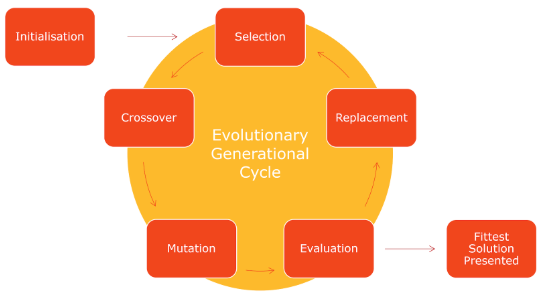
\includegraphics[width=7cm]{genetic_algorithm_circle.png}\\ \ \\
    \footnotesize{Genetic Algorithm Circle [3]}
\end{center}\\ 
\begin{figure}[h]
    \centering
    \label{genetic_algorithm_circle}
\end{figure}

\noindent \textbf{Steps of the Genetic Algorithm:}
\begin{itemize}
    \item \textbf{Initialization:}
    
    First, we must set up the genetic algorithm's first generation. Each individual, also known as a chromosome, stands for a potential neural network weight set that could be used to optimize the network. Each individual is simply a list of numbers or more lists. The problem determines the shape and type of these individuals. Since we are trying to train a neural network, we had to use continuous values even though the genetic algorithm performs better on discrete values. The shape of the chromosome is same with the shape of the neural network's weight set and the range of values is $[-100, 100]$. This range will be expanded at crossover step.
    
    \item \textbf{Evaluation:}
    
    The next step is to evaluate the individuals. We need a fitness function to determine if an individual is close to the solution or not. Higher fitness values are considered to make individuals better suited for survival and reproduction. We applied the loss function of the model as fitness function. When loss function is low then chromosome's fitness value is high.
    
    \item \textbf{Selection:}
    
    According to their fitness ratings, a certain number of people are chosen for reproduction in this step. The top n individuals which have high fitness values will be chosen.
    
    \item \textbf{Crossover:}

    In this step, two parents are selected from the selected individuals, and new individual is generated based on these parents. Since our individuals has continuous values, we choose a random value between the two corresponding values in individuals weight sets and assign it to the new individual. But if we use this method as described, we cannot expand the range we initially set. But the formula below expands the interval $[x_1, x_2]$ $10\%$ at each side.
    $$
    rand() * (x_1 - x_2) * 1.2 + x_2 * 1.1 - x_1 * 0.1
    $$
    \begin{center}
    \footnotesize{(Notice $rand()$ function returns number a between 0 and 1)}
    \end{center}
    
    Population size must be same as before after crossover step.

    Another important thing about crossing over is that some number of individuals passed to the next population without any crossover or mutation since it is not guaranteed that we will end up with better individuals after crossover. We do not want our population to have less fitness evaluation.

    
    \item \textbf{Mutation:}
    
    This state iterates over weight set of every individual and mutate the weight with some noise.
    
    \item \textbf{Replacement:}

    After all this steps, now we have newly generated population with same number of individuals. New population is at least as good as previous population because of the protected individuals.
    
    
    \item \textbf{Termination:}

    Termination condition can be based on the number of generations or some fitness threshold. If termination condition is met we can end the algorithm and return the individual with highest fitness value. If termination condition does not met we need to go back to evaluation step and keep doing the same steps until termination condition met.
\end{itemize}

By iteratively applying the steps of initialization, evaluation, selection, crossover, mutation, and replacement, the genetic algorithm explores the solution space and converges towards an optimal or near-optimal solution.

\section{\textbf{Experimental Evaluation}}
\subsection{Train Neural Network with Gradient Descent}

We use breast cancer data set from sklearn library as benchmark data set. It has 30 numerical features and 1 categorical target. 

First we need a base model to compare our models. Sequential neural network with 8 neurons in input layer, 16 neurons in hidden layer with relu activation and 1 output layer with sigmoid activation will do it.
\begin{center}
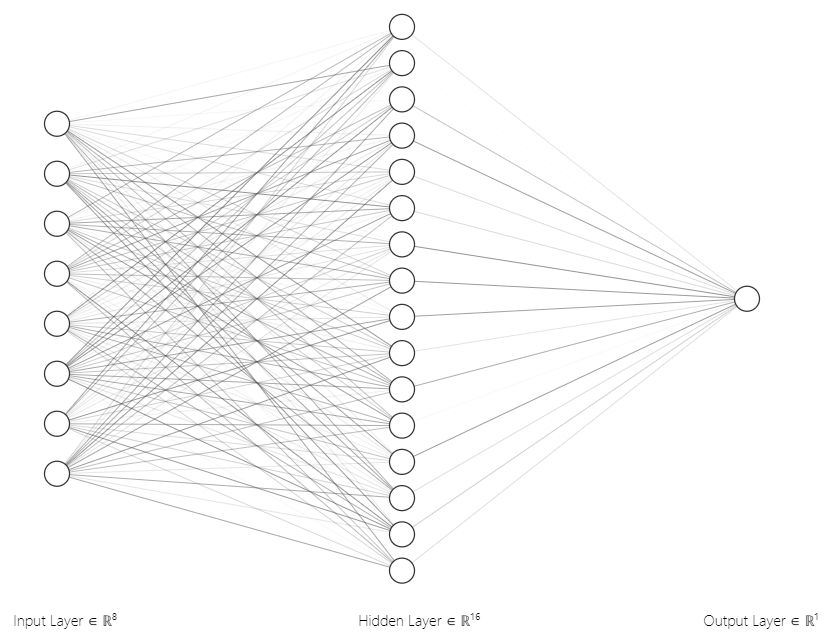
\includegraphics[width=5.6cm]{nn_architecture.png}\\
\footnotesize{Neural Network Architecture}
\end{center}\\ 

\begin{center}
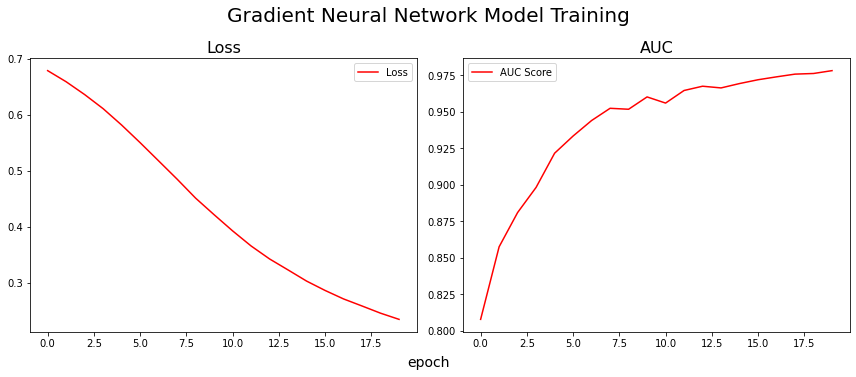
\includegraphics[width=7cm]{gradient_train.png}\\ \ \\
\footnotesize{Training with Gradient Descent}
\end{center}\\ 

\begin{center}
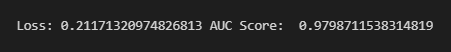
\includegraphics[width=7cm]{gradient_train_loss.png}\\ \ \\ 
\footnotesize{Loss After Training with Gradient Descent}
\end{center}\\ 

This result shows gradient descent does good job optimizing neural network.

\subsection{Train Neural Network with Genetic Algorithm}

When considering neural networks and non-gradient methods for optimization, the idea of training the network using a non-gradient algorithm is the first to come to mind. In the genetic algorithm, each individual represents a potential set of weights, and the objective is to find an optimal set of weights. After running the genetic algorithm for 100 generations with 200 chromosomes in each population, we were able to achieve a decrease in the loss function.

\begin{center}
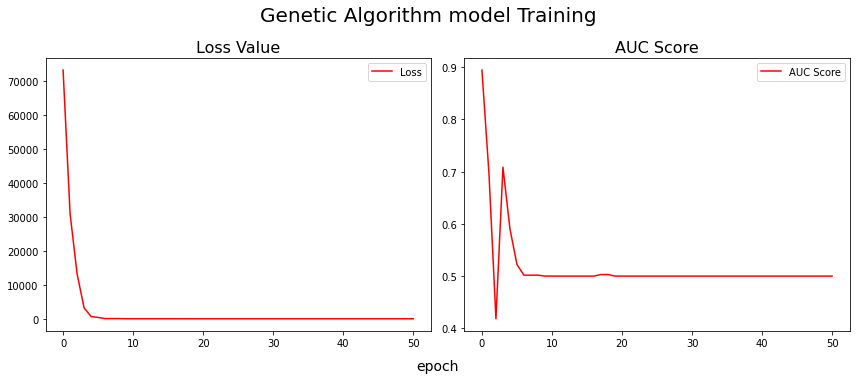
\includegraphics[width=7cm]{genetic_train.png}\\ \ \\
\footnotesize{Training with Genetic Algorithm}
\end{center}\\
\begin{center}
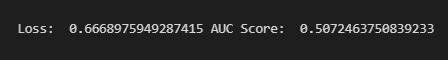
\includegraphics[width=7cm]{genetic_train_loss.png}\\ \ \\
\footnotesize{Loss After Training Genetic Algorithm}
\end{center}\\ 

However, the rate of loss decrease was not as much as desired. The primary reasons for this are the high dimensionality of the feature space and the complexity of the neural network's architecture. In contrast, the genetic algorithm performs well on simple linear regression or logistic regression models. However, in our case, the neural network has 409 adjustable real-valued parameters. This makes the training process more challenging to manage.

Furthermore, time complexity is a significant problem. Training the genetic algorithm required more time compared to gradient descent, which is a more commonly used optimization method for neural networks.

\subsection{Genetic Algorithm to Initialize Weights of Neural Network}

After training the weights with genetic algorithm all we need to do is to give this trained weights to model and train the parameters again with gradient descent. By doing this, we use genetic algorithm to find initial weights for neural network.

\begin{center}
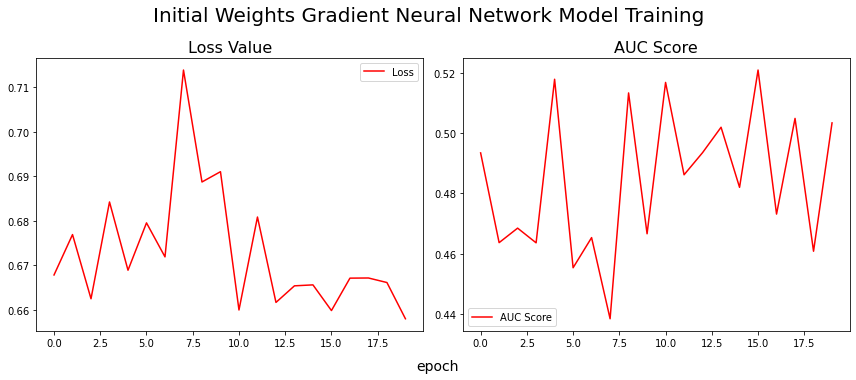
\includegraphics[width=7cm]{initial_weight_train.png}\\ \ \\ 
\footnotesize{Training Gradient Descent After Initialising weights}
\end{center}\\ 

\begin{center}
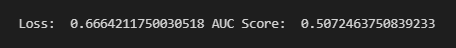
\includegraphics[width=7cm]{initial_weight_train_loss.png}\\ \ \\ 
\footnotesize{Loss After Training Gradient Descent with Initialised weights}
\end{center}\\ 

Loss changed a little. Model might stuck at local minimum.


\subsection{Simulated Annealing for Feature Selection}


Feature selection is a crucial step where we aim to identify the most relevant features from data. By doing this, we can improve model performance and reduce overfitting.

In the context of using simulated annealing for feature selection, the cost function represents the performance measure of model using a feature subset. During the process, the algorithm iteratively evaluates the performance of each feature subset. Then, it accepts or rejects new solutions based on a probability function which depends on the cost difference and a temperature parameter.

In our experiments, we conducted a comparison among  simulated annealing, random feature selection and utilizing all features. Based on the results, even our data is already preprocessed, we found that feature selection with simulated annealing is slightly better than random feature selection and almost same as utilizing all features.

\begin{center}
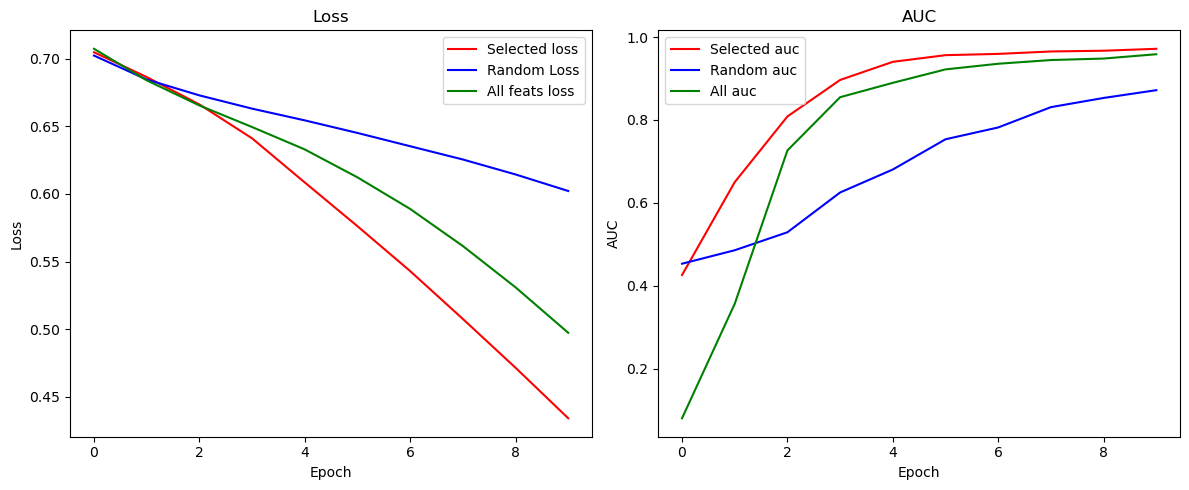
\includegraphics[width=7cm]{sa_ocmparison.png}\\ \ \\ 
\footnotesize{Comparison of different methods}
\end{center}\\ 


In this experiment, we utilized default hyperparameters. To ensure robustness, each iteration of the simulated annealing algorithm was repeated three times, and the average AUC score was obtained.

Since the relatively small of size dataset is used, the high level of randomness introduced some variability in the performance rankings.  However, despite this variability, the overall pattern of the experimental results demonstrates that simulated annealing is a promising method for feature selection.

\subsection{Genetic Algorithm and Simulated Annealing Together}
We will try to combine these three methods to train Neural Network.
\subsubsection{Hyper-parameter selection}
\ 

Both techniques require for a specific set of hyperparameters to be chosen by the programmer. We check every potential combination of perparameters and evaluated the objective function in order to determine the ideal combination.

\subsubsection{Feature selection with simulated annealing}
\

We did feature selection with simulated annealing using tuned hyperparameters.
\subsubsection{Initial weight selection with genetic algorithm}
\

We trained genetic algorithm with chosen hyperparameters and chosen features by simulated annealing. 

\subsubsection{Train gradient descent on neural network}
\ 
Gradient descent could not decrease the loss since initial weights stuck at local minima

\section{Conclusion}
\ 
Gradient-free methods are more effective for small search spaces. If search space get bigger, method may take more time and can even not converge to any good solution. 

Still they are good for hyper-parameter search and problems where we need to optimize non-differentiable or discontinues functions.

\begin{thebibliography}{00}
\bibitem{b1} https://www.example.com/
\bibitem{b2} https://www.researchgate.net/
\bibitem{b4} https://devforum.roblox.com/
\end{thebibliography}

\end{document}
